\documentclass{article}

\include{common}

\title{Classes}
\date{}

\begin{document}

\maketitle

\section{Data Abstraction}


An abstraction of a concept attempts to capture the essence of the concept -- its essential properties and behaviors -- by ignoring irrelevant details.
\begin{itemize}
\item Process abstraction - group the operations of a process in a subprogram and expose only the essential elements of the process to clients through the subprogram signature (e.g., function/method name and parameters)
\item Data abstraction - encapsulation of data with the operations defined on the data
\item A particular data abstraction is called an {\em abstract data type}.  Note that ADT's include process abstractions as well
\end{itemize}

In each case, an abstraction hides details --- details of a process or details of a data structure.

\begin{quote}
``Abstraction is selective ignorance.''\\
-- Andrew Koenig (C++ Guru)
\end{quote}


\section{A Complex Number ADT}


{\bf ADT: Complex}\\
Data:
\begin{itemize}
\item {\bf real: double} the real part of a complex number
\item {\bf imaginary: double} the imaginary part of a complex number
\end{itemize}
Operations:
\begin{itemize}
\item {\bf new} - construct a new complex number
\item {\bf plus} - add one complex number to another, yielding a new complex number
\end{itemize}
An ADT is {\it abstract} because the data and operations of the ADT are defined independently of how they are implemented.  We say that an ADT {\it encapsulates} the data and the operations on the data.





\section{Data Abstractions with Classes}

Java provides langauge suppport for defining ADTs in the form of classes.\\

A class is a blueprint for objects.  A class definition contains
\begin{itemize}
\item instance variables, a.k.a. member variables or fields -- the state, or data of an object
\item methods, a.k.a. member functions or messages -- the operations defined on objects of the class
\end{itemize}
We {\em instantiate} or {\em construct} an object from a class.





\section{Java Implementation of Complex Number ADT}\label{complex-class}


Here's a Java implementation of our complex number ADT \footnote{\url{http://introcs.cs.princeton.edu/java/33design/}}:

\begin{lstlisting}[language=Java]
public class Complex {
    // These are the data of the ADT

    private double real;
    private double imaginary;

    // These are the operations of the ADT

    public Complex(double aReal, double anImaginary) {
        real = aReal;
        imaginary = anImaginary;
    }

    public Complex plus(Complex other) {
        double resultReal = this.real + other.real;
        double resultImaginary = this.imaginary + other.imaginary;
        return new Complex(resultReal, resultImaginary);
    }
}
\end{lstlisting}






\section{Reference Variables}


Consider the following code:
\begin{lstlisting}[language=Java]
Complex a = new Complex(1.0, 2.0);
Complex b = new Complex(3.0, 4.0);
Complex c = a.plus(b);
\end{lstlisting}

{\tt a}, {\tt b}, and {\tt c} are {\it reference} variables of type {\tt Complex}.  Reference variables have one of two values:

\begin{itemize}
\item the address of an object in memory (in this case an instance of {\tt Complex}), or
\item {\tt null}, meaning the variable references nothing.
\end{itemize}





\section{Invoking Constructors}


The line:
\begin{lstlisting}[language=Java]
Complex a = new Complex(1.0, 2.0);
\end{lstlisting}

invokes the {\tt Complex} constructor, passing arguments {\tt 1.0} and {\tt 2.0}:

\begin{lstlisting}[language=Java,escapechar=`]
public Complex(aReal=`\colorbox{yellow}{1.0}`, anImaginary=`\colorbox{yellow}{2.0}`) {
    real = `\colorbox{yellow}{1.0}`;
    imaginary = `\colorbox{yellow}{2.0}`;
}
\end{lstlisting}

which {\it instantiates} a {\tt Complex} object and stores its address in the variable {\tt a}:

\begin{lstlisting}[language=Java]
Complex a = new Complex(1.0, 2.0);
\end{lstlisting}
Constructors initialize objects.  After the line above, {\tt Complex} object {\tt a}'s instance variables have the values {\tt 1.0} and {\tt 2.0}.





\section{Visualizing Objects and Instantiation}

The object creation expression {\tt new Complex(1.0, 2.0)}
%% \begin{lstlisting}[language=Java]
%% new Complex(1.0, 2.0)
%% \end{lstlisting}
applies the {\tt Complex} blueprint defined by the class definition from slide %\ref{complex-class}:

\begin{center}
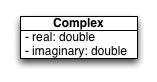
\includegraphics[height=.7in]{complex-class.png}
\end{center}

to the constructor arguments {\tt (1.0, 2.0)} to create an instance of {\tt Complex}:

\begin{center}
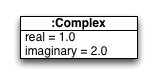
\includegraphics[height=.7in]{complex-instance.png}
\end{center}

We can assign this object to a reference variable, e.g.,\\ {\tt Complex a = new Complex(1.0, 2.0)}:
%% \begin{lstlisting}[language=Java]
%% Complex a = new Complex(1.0, 2.0);
%% \end{lstlisting}

\begin{center}
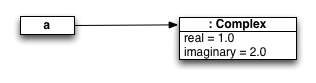
\includegraphics[height=.7in]{complex-reference.png}
\end{center}


\section{Invoking Methods on Objects}


The line:
\begin{lstlisting}[language=Java]
Complex c = a.plus(b);
\end{lstlisting}
invokes the {\tt plus} method on the {\tt a} object, passing the {\tt b} object as an argument, which binds the object referenced by {\tt b} to the parameter {\tt other}:
\begin{lstlisting}[language=Java,escapechar=`]
a.plus(other=`\colorbox{yellow}{b}`) {
  double resultReal = this.real + `\colorbox{yellow}{b}`.real; // 1.0 + 3.0
  double resultImaginary = this.imaginary + `\colorbox{yellow}{b}`.imaginary; // 2.0 + 4.0
  return new Complex(resultReal, resultImaginary);
}
\end{lstlisting}
which returns a new {\tt Complex} object and assigns its address to the  reference variable {\tt c}.

\section{Using the {\tt Complex} Class}

Users, or {\it clients} of the {\tt Complex} class can then write code like this:
\begin{lstlisting}[language=Java]
Complex a = new Complex(1.0, 2.0);
Complex b = new Complex(3.0, 4.0);
Complex c = a.plus(b);
\end{lstlisting}

without being concerned with {\tt Complex}'s implementation (which could use polar form, for example).  Clients (i.e., users) of the {\tt Complex} class need only be concerned with its interface, or {\it API} (application programmer interface) -- the public methods of the class.\\

After the code above we have the following {\tt Complex} objects in memory:
\begin{center}
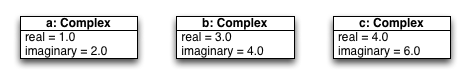
\includegraphics[height=.7in]{complex-abc.png}
\end{center}


\newpage

\section{The Anatomy of a Class Definition}


\begin{multicols}{2}

{\tt Card.java}

\begin{lstlisting}[language=Java]
import java.util.Arrays;

public class Card {

  public static final String[] VALID_RANKS = {"2", ... , "ace"};
  public static final String[] VALID_SUITS = {"diamonds", ... };
  private String rank;
  private String suit;

  public Card(String aRank, String aSuit) {
    // ...
  }
  public String toString() {
    return rank + " of " + suit;
  }
  private boolean isValidRank(String someRank) { ... }
}
\end{lstlisting}

\columnbreak

A class definition file contains

\begin{itemize}
\item import statements

\item class declaration

\item static variable definitions

\item instance variable definitions

\item constructor

\item public methods

\item private helper methods
\end{itemize}

\end{multicols}





\section{A Card Class, v0}



Consider how to represent a Card ADT:
\begin{itemize}
\item rank - the rank of a playing card, e.g., 2, jack, ace
\item suit - the suit of a playing card, e.g., spades, diamonds
\end{itemize}

\begin{lstlisting}[language=Java]
public class Card0 {

    String rank;
    String suit;
}
\end{lstlisting}

\begin{itemize}
\item {\tt rank} and {\tt suit} are instance variables
\item Every {\it instance} of {\tt Card0} has its own copy of instance variables.
\end{itemize}





\section{Using {\tt Card0}}



\begin{lstlisting}[language=Java]
public class Card0 {

    String rank;
    String suit;

    public static void main(String[] args) {
        Card0 c = new Card0();
        System.out.println(c);
    }
}
\end{lstlisting}

Note that we can put a {\tt main} method in any class. This is useful for exploratory testing, like we're doing here.\\

The {\tt String} representation isn't very appealing.  (What does it print?)





\section{Card Class, v1}


\begin{lstlisting}[language=Java]
public class Card1 {

    String rank;
    String suit;

    public String toString() {
        return rank + " of " + suit;
    }
    public static void main(String[] args) {
        Card1 swedishPop = new Card1();
        swedishPop.rank = "ace";
        swedishPop.suit = "base";
        Card1 handy = new Card1();
        handy.rank = "jack";
        handy.suit = "all trades";
        System.out.println(swedishPop);
        System.out.println(handy);
    }
}
\end{lstlisting}

Now we have an ``ace of base'' card and a ``jack of all trades'' card.  But those aren't valid cards.






\section{Encapsulation: Card, v2}


Let's protect the instance variables by making them private:
\begin{lstlisting}[language=Java]
public class Card2 {

    private String rank;
    private String suit;

    public String toString() {
        return rank + " of " + suit;
    }

    public static void main(String[] args) {
        Card2 c = new Card2();
        c.rank = "ace";
        c.suit = "base";
        System.out.println(c);
    }
}
\end{lstlisting}

Why does this still compile?

\begin{itemize}
\item {\tt main} method still part of {\tt Card2} - has access to private parts
\end{itemize}
Let's make a dealer class to represent client code.





\section{A Dealer Class}\footnote{Our Dealer class plays the role that a Driver class often plays in your homework.}


(We'll synchronize the names of Dealer classes with the names of Card classes, so {\tt Dealer2} is meant to test {\tt Card2}.)
\begin{lstlisting}[language=Java]
public class Dealer2 {

    public static void main(String[] args) {
        Card2 c = new Card2();
        c.rank = "ace";
        c.suit = "base";
        System.out.println(c);
    }
}
\end{lstlisting}

This won't compile (which is what we want). Why?





\section{Mutators: Card, v3}

\begin{lstlisting}[language=Java]
public class Card3 {

    private String rank;
    private String suit;

    public void setRank(String rank) {
        rank = rank;
    }
    public void setSuit(String suit) {
        suit = suit;
    }
}
\end{lstlisting}
\begin{itemize}
\item Now client code can set the rank and suit of a card by calling {\tt setRank} and {\tt setSuit}.
\item {\tt setX} is the Java convention for a setter method for an instance variable named {\tt x}.
\end{itemize}





\section{Dealing {\tt Card3}}


Let's try out our new {\tt Card3} class.
\begin{lstlisting}[language=Java]
public class Dealer3 {

    public static void main(String[] args) {
        Card3 c = new Card3();
        c.setRank("ace");
        c.setSuit("base");
        System.out.println(c);
    }
}
\end{lstlisting}

Oops.  Prints ``null of null''.  Why?






\section{Shadowing Variables}


The parameters in the setters ``shadowed'' the instance variables:
\begin{lstlisting}[language=Java]
public void setRank(String rank) {
    rank = rank;
}

public void setSuit(String suit) {
    suit = suit;
}
\end{lstlisting}

\begin{itemize}
\item {\tt rank} in {\tt setRank} refers to the local {\tt rank} variable, not the instance variable of the same name
\item {\tt suit} in {\tt setSuit} refers to the local {\tt suit} variable, not the instance variable of the same name
\end{itemize}






\section{Dealing with {\tt this}: Card, v4}

\begin{lstlisting}[language=Java]
public class Card4 {
    private String rank;
    private String suit;

    public void setRank(String rank) {
        this.rank = rank;
    }

    public void setSuit(String suit) {
        this.suit = suit;
    }
}
\end{lstlisting}

\begin{itemize}
\item Every instance of a class has a {\tt this} reference which refers to the instance on which a method is being called.
\item {\tt this.rank} refers to the {\tt rank} instance variable for the {\tt Card4} instance on which {\tt setRank} is being called.
\item {\tt this.rank} is different from the local {\tt rank} variable that is a parameter to the {\tt setRank} method.
\end{itemize}





\section{Dealing {\tt Card4}}


\begin{lstlisting}[language=Java]
public class Dealer4 {

    public static void main(String[] args) {
        Card4 c = new Card4();
        c.setRank("ace");
        c.setSuit("base");
        System.out.println(c);
    }
}
\end{lstlisting}

Now we have encapsulation, but we can still create invalid {\tt Card4}s, e.g., ``base'' is not a valid suit.  How to fix?





\section{Class Invariants}


Class invariant: a condition that must hold for all instances of a class in order for instances of the class to be considered valid.\\

Invariants for Card class:
\begin{itemize}
\item {\tt rank} must be one of \{{\tt "2", "3", "4", "5", "6", "7", "8", "9",
         "10", "jack", "queen", "king", "ace"}\}
\item {\tt suit} must be one of \{{\tt "diamonds", "clubs", "hearts","spades"}\}
\end{itemize}






\section{Maintaining Class Invariants via Input Validation}



{\tt rank} invariant can be maintained by adding:

\begin{lstlisting}[language=Java]
public class Card5 {
    private final String[] VALID_RANKS =
        {"2", "3", "4", "5", "6", "7", "8", "9",
         "10", "jack", "queen", "king", "ace"};
    public void setRank(String rank) {
        if (!isValidRank(rank)) {
            System.out.println(rank + " is not a valid rank.");
            System.exit(0);
        }
        this.rank = rank;
    }
    private boolean isValidRank(String someRank) {
        return contains(VALID_RANKS, someRank);
    }
    private boolean contains(String[] array, String item) {
        for (String element: array) {
            if (element.equals(item)) {
                return true;
            }
        }
        return false;
    }
    // ...
}
\end{lstlisting}





\section{Class Invariants Ensure Consistent Objects}


Now we can't write code that instantiates an invalid {\tt Card5} object:
\begin{lstlisting}[language=Java]
public class Dealer5 {

    public static void main(String[] args) {
        Card5 c = new Card5();
        c.setRank("ace");
        c.setSuit("base");
        System.out.println(c);
    }
}
\end{lstlisting}
yields:
\begin{lstlisting}[language=bash]
$ java Dealer5
base is not a valid suit.
\end{lstlisting}
%$ - get Emacs to stop displaying stuff below in pink


\section{Progress Check}


Let's review our progress with our Card class design:
\begin{itemize}
\item We have a nice string representation of Card objects ({\tt Card1}).
\item We have encapsulated the rank and suit in private instance variables ({\tt Card2}) with mutator methods ({\tt Card4}) to set their values.
\item We validate the rank and suit in the mutator methods so we can't set invalid ranks and suits in Card objects ({\tt Card5}).
\end{itemize}







\section{Classes and Objects}


{\tt Card5} now ensures that we don't create card objects with invalid ranks or suits.
But consider this slight modification to {\tt Dealer5}:
\begin{lstlisting}[language=Java,mathescape=true]
public class Dealer5 {

    public static void main(String[] args) {
        Card5 c = new Card5();
        ${\mathbf System.out.println(c);}$
        c.setRank("ace");
        c.setSuit("base");
        System.out.println(c);
    }
}
\end{lstlisting}

What if we printed our {\tt Card5} instance, {\tt c}, before we called the setters?





\section{Object Initialization}


There are two ways to initialize the instance variables of an object:
\begin{itemize}
\item Declaration point initialization:
\begin{lstlisting}[language=Java,mathescape=true]
public class Card {
  private String rank = "2";
  // ...
}
\end{lstlisting}
\item Constructors
\begin{lstlisting}[language=Java,mathescape=true]
public class Card {
  public Card() {
    rank = "2";
  }
  // ...
}
\end{lstlisting}

\end{itemize}
A constructor is what's being called when you invoke operator {\tt new}.




\section{Initializing Objects}


Since we didn't write our own constructor, Java provided a default no-arg constructor that simply sets instance variables (that don't have their own declaration-point intializations) to their default values.  That's why {\tt Card5} objects are {\tt null of null} after they're instantiated.  We have to call the setters on a {\tt Card5} instance before we have a valid object.\\


In general, it's poor style to require multi-step initialization.
\begin{itemize}
\item After {\tt new Card5()} is called, instance variables have useless defaults.
\item Client programmer must remember to call setter methods.
\item Often there can be order dependencies that we don't want to burden client programmers with.
\end{itemize}
The way to fix this is by writing our own constructor.





\section{A Card Constructor}


If we write a constructor, Java won't provide a default no-arg constructor. (We may choose to provide one.)
\begin{lstlisting}[language=Java]
public class Card6 {
    // ...
    public Card6(String rank, String suit) {
        setRank(rank);
        setSuit(suit);
    }
    // ...
}
\end{lstlisting}

Now we have a safer, more consistent  way to initialize objects:
\begin{lstlisting}[language=Java]
public class Dealer6 {

    public static void main(String[] args) {
        Card6 c = new Card6("queen", "hearts");
        System.out.println(c);
    }
}
\end{lstlisting}





\section{Static Members}


Do we need a separate instance of {\tt VALID\_RANKS} and {\tt VALID\_SUITS} for each instance of our Card class?

{\tt static} members are shared with all instances of a class:
\begin{lstlisting}[language=Java]
public static final String[] VALID_RANKS =
    {"2", "3", "4", "5", "6", "7", "8", "9",
     "10", "jack", "queen", "king", "ace"};
public static final String[] VALID_SUITS =
    {"diamonds", "clubs", "hearts","spades"};
\end{lstlisting}
Given the declarations above:
\begin{itemize}
\item Each instance shares a single copy of {\tt VALID\_RANKS} and a single copy of {\tt VALID\_SUITS}
\item Since they're {\tt final}, we can safely make them {\tt public} so clients of our Card class can use them
\end{itemize}





\section{One Final Enhancement}

{\tt Card6} is pretty good, but we can write code like this:

\begin{lstlisting}[language=Java]
public class Dealer6 {

    public static void main(String[] args) {
        Card6 c = new Card6("queen", "hearts");
        System.out.println(c);
        c.setRank("jack"); // modifying c
        System.out.println(c);
    }
}
\end{lstlisting}
Does this make sense?  Should Card objects be mutable?





\section{Immutable Objects}


Card objects don't change.  We can model this behavior by removing the setters and putting the initialization code in the constructor (or making the setters private and calling them from the constructor):

\begin{lstlisting}[language=Java]
public Card(String aRank, String aSuit) { // constructor
  if (!isValidRank(rank)) {
    System.out.println(aRank + " is not a valid rank.");
    System.exit(0);
  }
  rank = aRank;
  if (!isValidSuit(aSuit)) {
    System.out.println(aSuit + " is not a valid suit.");
    System.exit(0);
  }
  suit = aSuit;
}
\end{lstlisting}

\small Note the use of another idiom for disambiguating constructor paramters from instance variables (as opposed to using {\tt this}).\normalsize





\section{Designing Immutable Classes}


An immutable class is a class whose instances cannot be modified.  To make a class immutable:

\begin{itemize}
\item Don't provide mutator methods (``setters'')
\item Make the class {\tt final} so it can't be extended (there's another way to accomplish this, but making the class {\tt final} is good enough for now)
\item Make all fields {\tt final}
\item Make all fields {\tt private}
\item For fields of mutable class types, return defensive copies in accessor methods (we'll discuss this later)
\end{itemize}





\section{Prefer Immutable Classes}


In general, make your classes immutable unless you have a good reason to make them mutable.  Why?  Because immutable objects
\begin{itemize}
\item are simpler to design because you don't have to worry about enforcing class invariants in multiple places,
\item are easier to reason about because the state of an object never changes after instantiation,
\item are inherently thread-safe because access to mutable data need not be syncronized, and
\item enable safe instance sharing, so redundant copies need not be created.
\end{itemize}





\section{A Few Final Bits of Polish}


Take a look at the final evolution of our Card class, \href{https://github.com/cs1331/cs1331.github.io/blob/master/code/classes/Card.java}{Card.java}.  It contains a few more enhancements:
\begin{itemize}
\item Instead of simply terminating the program, the constructor throws {\tt IllegalArgumentException} on invalid input so that client code can choose to deal with the exception at run-time.
\item Input is normalized to lower case and spaces trimmed to make the Card object robust to oddly formatted input.
\item It has an {\tt equals()} method.
\end{itemize}






\section{Equality}

\begin{itemize}
\item {\tt ==} means identity equality (aliasing) for reference types (objects).
\item The {\tt equals(Object)} tests value equality for objects.
\end{itemize}

Given our finished \href{https://github.com/cs1331/cs1331.github.io/blob/master/code/classes/Card.java}{Card.java} class with a properly implemented {\tt equals(Object)} method, this code:

\begin{lstlisting}[language=Java]
  Card c1 = new Card("ace", "spades");
  Card c2 = new Card("ace", "spades");
  Card c3 = c1;
  System.out.println("c1 == c2 returns " + (c1 == c2));
  System.out.println("c1.equals(c2) returns " + c1.equals(c2));
  System.out.println("c1 == c3 returns " + (c1 == c3));
  System.out.println("c1.equals(c3) returns " + c1.equals(c3));
\end{lstlisting}

produces this output:

\begin{lstlisting}[language=Java]
  c1 == c2 returns false
  c1.equals(c2) returns true
  c1 == c3 returns true
  c1.equals(c3) returns true
\end{lstlisting}

{\small By the way, what if we left off the parentheses around {\tt c1 == c2} in  {\tt System.out.println("c1 == c2 returns " + (c1 == c2))}}?





\section{Review Question 1}

\begin{lstlisting}[language=Java]
public class Kitten {
    private String name;

    public Kitten(String name) {
        name = name;
    }
    public String toString() {
        return "Kitten: " + name;
    }
}
\end{lstlisting}

Assume the following statements have been executed:

\begin{lstlisting}
        Kitten maggie = new Kitten("Maggie");
        Kitten fiona = new Kitten("Fiona");
        Kitten fiona2 = new Kitten("Fiona");
\end{lstlisting}

What is the value of {\tt maggie}?
\begin{itemize}
\itemsep0em
\item ?
\end{itemize}




\section{Review Question 1 Answer}

\begin{lstlisting}[language=Java]
public class Kitten {
    private String name;

    public Kitten(String name) {
        name = name;
    }
    public String toString() {
        return "Kitten: " + name;
    }
}
\end{lstlisting}

Assume the following statements have been executed:

\begin{lstlisting}
        Kitten maggie = new Kitten("Maggie");
        Kitten fiona = new Kitten("Fiona");
        Kitten fiona2 = new Kitten("Fiona");
\end{lstlisting}

What is the value of {\tt maggie}?
\begin{itemize}
\itemsep0em
\item the address of a {\tt Kitten} object
\end{itemize}




\section{Review Question 2}

\begin{lstlisting}[language=Java]
public class Kitten {
    private String name;

    public Kitten(String name) {
        name = name;
    }
    public String toString() {
        return "Kitten: " + name;
    }
}
\end{lstlisting}

Assume the following statements have been executed:

\begin{lstlisting}
        Kitten maggie = new Kitten("Maggie");
        Kitten fiona = new Kitten("Fiona");
        Kitten fiona2 = new Kitten("Fiona");
\end{lstlisting}

What does {\tt maggie.toString()} return?
\begin{itemize}
\itemsep0em
\item ?
\end{itemize}




\section{Review Question 2 Answer}

\begin{lstlisting}[language=Java]
public class Kitten {
    private String name;

    public Kitten(String name) {
        name = name;
    }
    public String toString() {
        return "Kitten: " + name;
    }
}
\end{lstlisting}

Assume the following statements have been executed:

\begin{lstlisting}
        Kitten maggie = new Kitten("Maggie");
        Kitten fiona = new Kitten("Fiona");
        Kitten fiona2 = new Kitten("Fiona");
\end{lstlisting}

What does {\tt maggie.toString()} return?
\begin{itemize}
\itemsep0em
\item {\tt "Kitten: null"}
\end{itemize}




\section{Review Question 3}

\begin{lstlisting}[language=Java]
public class Kitten {
    private String name;

    public Kitten(String name) {
        name = name;
    }
    public String toString() {
        return "Kitten: " + name;
    }
}
\end{lstlisting}

Assume the following statements have been executed:

\begin{lstlisting}
        Kitten maggie = new Kitten("Maggie");
        Kitten fiona = new Kitten("Fiona");
        Kitten fiona2 = new Kitten("Fiona");
\end{lstlisting}

What is the value of the expression {\tt fiona == fiona2}?
\begin{itemize}
\itemsep0em
\item ?
\end{itemize}




\section{Review Question 3 Answer}

\begin{lstlisting}[language=Java]
public class Kitten {
    private String name;

    public Kitten(String name) {
        name = name;
    }
    public String toString() {
        return "Kitten: " + name;
    }
}
\end{lstlisting}

Assume the following statements have been executed:

\begin{lstlisting}
        Kitten maggie = new Kitten("Maggie");
        Kitten fiona = new Kitten("Fiona");
        Kitten fiona2 = new Kitten("Fiona");
\end{lstlisting}

What is the value of the expression {\tt fiona == fiona2}?
\begin{itemize}
\itemsep0em
\item {\tt false}
\end{itemize}




\section{Review Question 4}

\begin{lstlisting}[language=Java]
public class Kitten {
    private String name;

    public Kitten(String name) {
        name = name;
    }
    public String toString() {
        return "Kitten: " + name;
    }
}
\end{lstlisting}

Assume the following statements have been executed:

\begin{lstlisting}
        Kitten maggie = new Kitten("Maggie");
        Kitten[] kittens = new Kitten[5];
\end{lstlisting}

What is the value of {\tt kittens[0]} ?
\begin{itemize}
\itemsep0em
\item ?
\end{itemize}




\section{Review Question 4 Answer}

\begin{lstlisting}[language=Java]
public class Kitten {
    private String name;

    public Kitten(String name) {
        name = name;
    }
    public String toString() {
        return "Kitten: " + name;
    }
}
\end{lstlisting}

Assume the following statements have been executed:

\begin{lstlisting}
        Kitten maggie = new Kitten("Maggie");
        Kitten[] kittens = new Kitten[5];
\end{lstlisting}

What is the value of {\tt kittens[0]} ?
\begin{itemize}
\itemsep0em
\item {\tt null}
\end{itemize}



\end{document}
